\documentclass[12pt]{article}

\usepackage{tikz}
\usepackage{amsmath}
\usepackage{graphicx}
\usepackage{tabularx}
\usepackage{multicol}
\usepackage{algpseudocode}
\usepackage{algorithm}

% Geometry 
\usepackage{geometry}
\geometry{letterpaper, left=15mm, top=20mm, right=15mm, bottom=20mm}

% Fancy Header
\usepackage{fancyhdr}
\renewcommand{\footrulewidth}{0.4pt}
\pagestyle{fancy}
\fancyhf{}
\chead{CSC 360 - Analysis of Algorithms}
\lfoot{CALU Fall 2021}
\rfoot{RDK}

% Add vertical spacing to tables
\renewcommand{\arraystretch}{1.4}

% Macros
\newcommand{\definition}[1]{\underline{\textbf{#1}}}

\newenvironment{rcases}
  {\left.\begin{aligned}}
  {\end{aligned}\right\rbrace}

% Begin Document
\begin{document}

\section*{Notes Week 8}

\begin{itemize}

    \item A \definition{loop} is an edge that connects a node to itself. Mostly relevant to directed graphs \\
    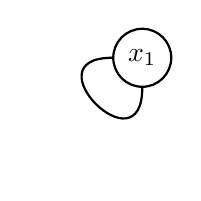
\begin{tikzpicture}[node distance={15mm}, thick, main/.style = {draw, circle}] 
        \node[main] (1) {$x_1$};  
        \draw (1) to [out=180,in=270,looseness=5] (1);  
    \end{tikzpicture}

    \item A \definition{simple path} is a path where all vertices are distinct except possibly the first and last. \\
    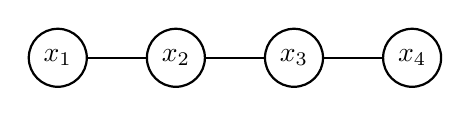
\begin{tikzpicture}[node distance={15mm}, thick, main/.style = {draw, circle}] 
        \node[main] (1) {$x_1$};  
        \node[main] (2) [right of = 1] {$x_2$};  
        \node[main] (3) [right of = 2] {$x_3$};  
        \node[main] (4) [right of = 3] {$x_4$};  
        \draw (1) -- (2);  
        \draw (3) -- (4);  
        \draw (2) -- (3);  
    \end{tikzpicture}

    \item A \definition{cycle} is a path that starts and ends on the same vertex.

    \item \definition{Acyclic} graphs contain no cycles.

    \item \definition{DAG}: Directed Acyclic Graph

    \item \definition{Strongly} connected graphs are ones where any vertex has a path to any other vertex; \definition{Weakly} connected graphs have vertices without paths to other vertices.

    \item A \definition{Bipartite Graph} is one we can separate vertices into two groups where edges only travel between groups. \\
    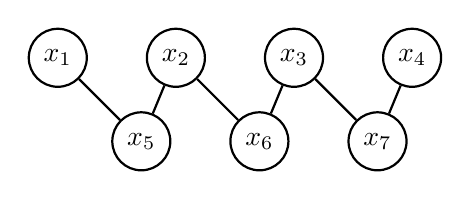
\begin{tikzpicture}[node distance={15mm}, thick, main/.style = {draw, circle}] 
        \node[main] (1) {$x_1$};  
        \node[main] (2) [right of = 1] {$x_2$};  
        \node[main] (3) [right of = 2] {$x_3$};  
        \node[main] (4) [right of = 3] {$x_4$};
        \node[main] (5) [below right of = 1] {$x_5$};
        \node[main] (6) [below right of = 2] {$x_6$};
        \node[main] (7) [below right of = 3] {$x_7$};  
        \draw (1) -- (5);
        \draw (2) -- (5);
        \draw (2) -- (6);
        \draw (3) -- (6);
        \draw (3) -- (7);
        \draw (4) -- (7);  
    \end{tikzpicture} 

    \item Formally, a \definition{Bipartite Graph} is $BG = (A \cup B, E)$ such that every edge connects an element of A with an element B.
    
    \item A complete Bipartite graph is one where all nodes in group B are connected to all nodes in group B.

    \item A \definition{Tree} is any connected, undirected, acyclic graph.

\end{itemize}

\pagebreak

\section*{Depth-First $vs$ Breadth-First Searches}

\begin{tabularx}{\textwidth}{X X}

    \definition{Depth-First Search}

    \begin{enumerate}

        \item Push Start Vertex
        \item Mark start vertex as visited
        \item Loop until stack empty
        \begin{enumerate}
            \item Pop $U$
            \item Mark $U$ as visited
            \item For each of $U$ unvisited neighbors, push them
        \end{enumerate}

    \end{enumerate}

    &

    \definition{Breadth-First Search}

    \begin{enumerate}

        \item Enqueue Start Vertex
        \item Mark start vertex as visited
        \item Loop until queue empty
        \begin{enumerate}
            \item Dequeue $U$
            \item Mark $U$ as visited
            \item For each of $U$ unvisited neighbors, Enqueue them
        \end{enumerate}

    \end{enumerate}

\end{tabularx}

\begin{itemize}

    \item Both BFS and DFS are $O(V + E)$
    \begin{itemize}
        \item Vertices: $V = n$
        \item Edges: $E = n(n-1)/2$ at most in a complete, undirected graph
        \item Therefore: $O(n + n^2) = O(n^2)$ as an upper bound, but is dependet on
    \end{itemize}

    \item Under what circumstances would BFS or DFS run faster?

    \item Well, neither? Closer on graph favors BFS.

\end{itemize}

\section*{Topological Sort}

\begin{itemize}

    \item An ordering of vertices in a directed, acyclic graph such that, if there is a path, from vertex $A$ to vertex $B$, then vertex $B$ appears after vertex $A$ in the order. \\
    
\end{itemize}

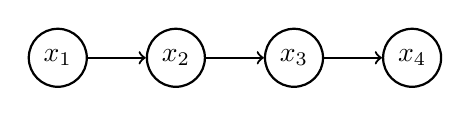
\begin{tikzpicture}[node distance={15mm}, thick, main/.style = {draw, circle}] 
        \node[main] (1) {$x_1$};
        \node[main] (2) [right of = 1] {$x_2$};
        \node[main] (3) [right of = 2] {$x_3$};
        \node[main] (4) [right of = 3] {$x_4$};
        \draw[->] (1) -- (2);
        \draw[->] (3) -- (4);
        \draw[->] (2) -- (3);
\end{tikzpicture}

\begin{itemize}

    \item Topological sorts are not guaranteed to be unique. There could be many correct orders.

    \item Examples: Family Tree, Course Prerequisites

    \item Assumptions:
    \begin{enumerate}
        \item Indegree for each vertex is stored
        \item Edges stored in an adjacency list
    \end{enumerate}

\end{itemize}

\pagebreak

\begin{algorithm}
    \caption{Topological Sort 1 $O(n^2)$}
    \begin{algorithmic}
        \While{Graph is not empty}
            \State Find any vertex with no incoming edges
            \State Display Vertex
            \State Remove it, and its edges, from the graph
        \EndWhile
    \end{algorithmic}
\end{algorithm}

\begin{algorithm}
    \caption{Topological Sort 2}
    \begin{algorithmic}
        \State Maintain a queue of vertices with indegree $0$
        \While Queue is not empty
            \State Dequeue a vertex
            \State Display the Vertex
            \State Remove it and its edges from the graph
            \State Update remaining Vertices, enqueueing any whose indgree is $0$
        \EndWhile
    \end{algorithmic}
\end{algorithm}

\begin{itemize}
    \item Each vertex enqueued and dequeued once $\rightarrow O(n^2)$
    \item Each edge gets removed once $\rightarrow n^2$ potential
    \item Therefore, Topological Sort 2 is $O(V+E)$
    \item TS2 depends on number of edges, whereas TS1 depends on nodes
    \item TS2 approaches TS1 only when the graph is complete, or close to it
\end{itemize}

\section*{The Selection Problem}

Find the $k^{th}$ largest number in a set of $n$ numbers.

\begin{itemize}

    \item \definition{$i^{th}$ order statistic}: the $i^{th}$ smallest term in a set of $n$ elements
    \item Recall week 1 notes; best algorithm was $O(nlog(n))$
    \item It's possible to make this $O(n)$
    \begin{itemize}
        \item Pick a good pivot similar to QuickSort
        \item Then like Binary Search, use the half that's relevant
        \item The dividing runs in $(log(n))$ but the pivot search runs in $O(n)$
    \end{itemize}

\end{itemize}


\end{document}